\subsubsection{Waiting time} \label{sec:waiting_time}

Waiting time is the amount of time that individuals from either type wait in 
waiting zone 1 so that they can receive their service. 
For a given set of parameters there are three different performance measures 
around the mean waiting time that can be calculated; the mean waiting time of
type 1 individuals:

\begin{equation} \label{eq:closed_form_waiting_type_1}
    W^{(1)} = \frac{\sum_{\substack{(u,v) \, \in S_A^{(1)} \\ v \geq C}} 
    \frac{1}{C \mu} \times (v-C+1) \times \pi(u,v)}{\sum_{(u,v) \, 
    \in S_A^{(1)}} \pi(u,v)}
\end{equation}

The mean waiting time of type 2 individuals:

\begin{equation}\label{eq:closed_form_waiting_type_2}
    W^{(2)} = \frac{\sum_{\substack{(u,v) \, \in S_A^{(2)} \\ min(v,T) \geq C}} 
    \frac{1}{C \mu} \times (\min(v+1,T)-C) \times \pi(u,v)}{\sum_{(u,v) \, 
    \in S_A^{(2)}} \pi(u,v)}
\end{equation} 

The overall mean waiting time:

\begin{equation}\label{eq:overall_waiting_time}
    W = \frac{\lambda_1 P_{L'_1}}{\lambda_2 P_{L'_2} + \lambda_1 P_{L'_1}} W^{(1)} 
    + \frac{\lambda_2 P_{L'_2}}{\lambda_2 P_{L'_2} + \lambda_1 P_{L'_1}} W^{(2)}
\end{equation}
 
Here \(S_A^{(1)}\) and \(S_A^{(2)}\) are the set of accepting states for type
1 and type 2 individuals. These are the set of states that the model is able
to accept a specific type of individuals.

\begin{equation}\label{eq:accepting_states_type_1}
    S_A^{(1)} = \{(u, v) \in S \; | \; v < N \}
\end{equation}

\begin{equation}\label{eq:accepting_states_type_2}
    S_A^{(2)}=
    \begin{cases}
        \{(u, v) \in S \; | \; u < M \}, & \textbf{if } T \leq N\\
        \{(u, v) \in S \; | \; v < N \}, & \textbf{otherwise}
    \end{cases}
\end{equation}

Equation \ref{eq:overall_waiting_time} makes use of the proportion of type 1 
and type 2 individuals that are not lost to the system. These probabilities are 
given by \(P_{L'_1}\) and \(P_{L'_2}\) where:

\begin{equation}\label{eq:proportion_of_accepting_individuals}
    P_{L'_1} = \sum_{(u,v) \, \in S_A^{(1)}} \pi(u,v) \hspace{2cm}
    P_{L'_2} = \sum_{(u,v) \, \in S_A^{(2)}} \pi(u,v)
\end{equation}
 
Appendix \ref{sec:appendix_mean_waiting} gives more details on the recursive
formula that equations (\ref{eq:closed_form_waiting_type_1}),
(\ref{eq:closed_form_waiting_type_2}) and (\ref{eq:overall_waiting_time})
originate from. 

Figure \ref{fig:markov_vs_des_waiting_time_comparison} shows a comparison 
between the calculated mean waiting time using Markov chains and the simulated waiting time using discrete event simulation.

\begin{figure}[ht]
    \centering
    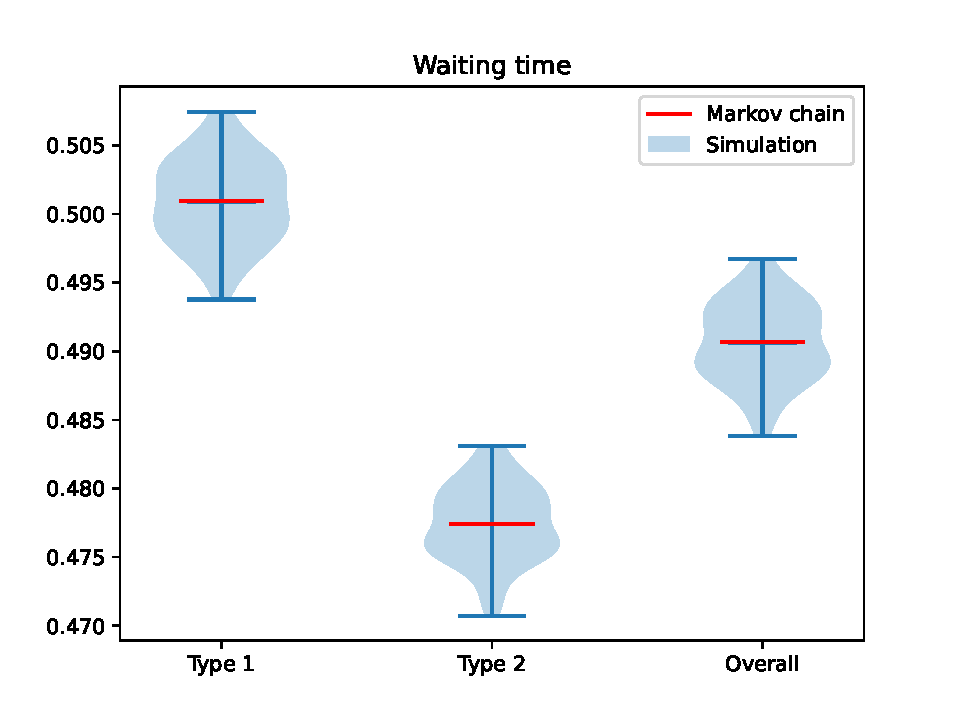
\includegraphics[width=\textwidth]{imgs/markov_vs_des/waiting_time/main.pdf}
    \caption{
        Comparison of mean waiting time between values obtained from the Markov
        chain formulas and values obtained from simulation. The simulation 
        was ran 100 times and the recorded mean waiting time at each iteration
        is used to populate the violin plots.
    }
    \label{fig:markov_vs_des_waiting_time_comparison}
\end{figure}
